\documentclass[conference]{IEEEtran}
\IEEEoverridecommandlockouts
% The preceding line is only needed to identify funding in the first footnote. If that is unneeded, please comment it out.
\usepackage{cite}
\usepackage{amsmath,amssymb,amsfonts}
\usepackage{algorithmic}
\usepackage{graphicx}
\usepackage{textcomp}
\usepackage{xcolor}
\usepackage{tabularx}
\usepackage{multirow}
\usepackage{graphics} % for pdf, bitmapped graphics files
\usepackage{subfig}
\usepackage{subcaption}
\usepackage{hyperref}
\usepackage{academicons}
\usepackage{xcolor}
\usepackage{listings}
\usepackage{tabularx} % Asegúrate de incluir este paquete

\usepackage{tikz}
\usetikzlibrary{shapes.geometric, arrows}

\usetikzlibrary{shapes.geometric, arrows}

\tikzstyle{startstop} = [rectangle, rounded corners, minimum width=3cm, minimum height=1cm,text centered, draw=black, fill=red!30]
\tikzstyle{process} = [rectangle, minimum width=3cm, minimum height=1cm, text centered, draw=black, fill=blue!30]
\tikzstyle{arrow} = [thick,->,>=stealth]


\def\BibTeX{{\rm B\kern-.05em{\sc i\kern-.025em b}\kern-.08em
		T\kern-.1667em\lower.7ex\hbox{E}\kern-.125emX}}

% Color Enlace
\definecolor{colorEnlace}{RGB}{0, 0, 0}
\hypersetup{
	colorlinks=true,
	linkcolor=colorEnlace,
	citecolor=colorEnlace,
	urlcolor=colorEnlace,
	pdfauthor={Davis Bremdow Salazar Roa},
	pdftitle={Sistemas Embebidos}
}
\lstset{
	language=C,
	basicstyle=\ttfamily\small,
	keywordstyle=\color{blue},
	stringstyle=\color{red},
	commentstyle=\color{green!60!black},
	showstringspaces=false,
	numbers=left,
	numberstyle=\tiny\color{gray},
	frame=none,
	breaklines=true,
	tabsize=1
}

% Control 
\usepackage{amsmath}
\begin{document}
	
	\title{Informe final - Amplificador Diferencial Retroalimentado}
	\author{
        \makebox[\textwidth][c]{\large\textbf{Universidad Nacional de San Antonio Abad del Cusco}}\\
        \makebox[\textwidth][c]{\normalsize\textit{Escuela profesional de Ingeniería Electrónica}}\\
		\makebox[\textwidth][c]{\normalsize\textit{Laboratorio de Circuitos Electrónicos III}}\\
        \and
        \IEEEauthorblockN{Miguel Angel Janqui Cavero}
        \IEEEauthorblockA{Ingeniero Electrónico \\
                Cusco, Perú \\
                miguel.janqui@unsaac.edu.pe}
        \and
        \IEEEauthorblockN{Ruth Juana Espino Puma - 185746}
        \IEEEauthorblockA{Estudiante de Ingeniería Electrónica \\
                Cusco, Perú \\
                184657@unsaac.edu.pe}
        \and
        \IEEEauthorblockN{Davis Bremdow Salazar Roa - 200353}
        \IEEEauthorblockA{Estudiante de Ingeniería Electrónica \\
                Cusco, Perú \\
                200353@unsaac.edu.pe}
	}
    
	\maketitle
    \begin{abstract}
		Los amplificadores retroalimentados son dispositivos electrónicos que incorporan una parte de la señal de salida de nuevo a su entrada con el objetivo de controlar y mejorar su comportamiento. Esta retroalimentación puede ser negativa, lo que estabiliza la ganancia, reduce la distorsión y amplía el ancho de banda, o positiva, que se utiliza en aplicaciones como osciladores.
	\end{abstract}
    \begin{IEEEkeywords}
		feedback, amplifier, gain, stability, bandwidth, distortion, negative, positive, op-amp, linearity
	\end{IEEEkeywords}

    \section{Análisis en alterna y parámetros de salida: T, Aif, Avf, Zif, Zof}

    El análisis a realizar para el amplificador diferencial se muestra en la figura \ref{fig:circuito-inicial} y es el que se tomara en cuenta para realizar el análisis en alterna, siendo este modificado mediante el agregado de una resistencia para poder obtener una correcta polarización en los transistores logrando mantener la señal de entrada con un ligero desfase.
    
    \begin{figure}[h]
        \centering
        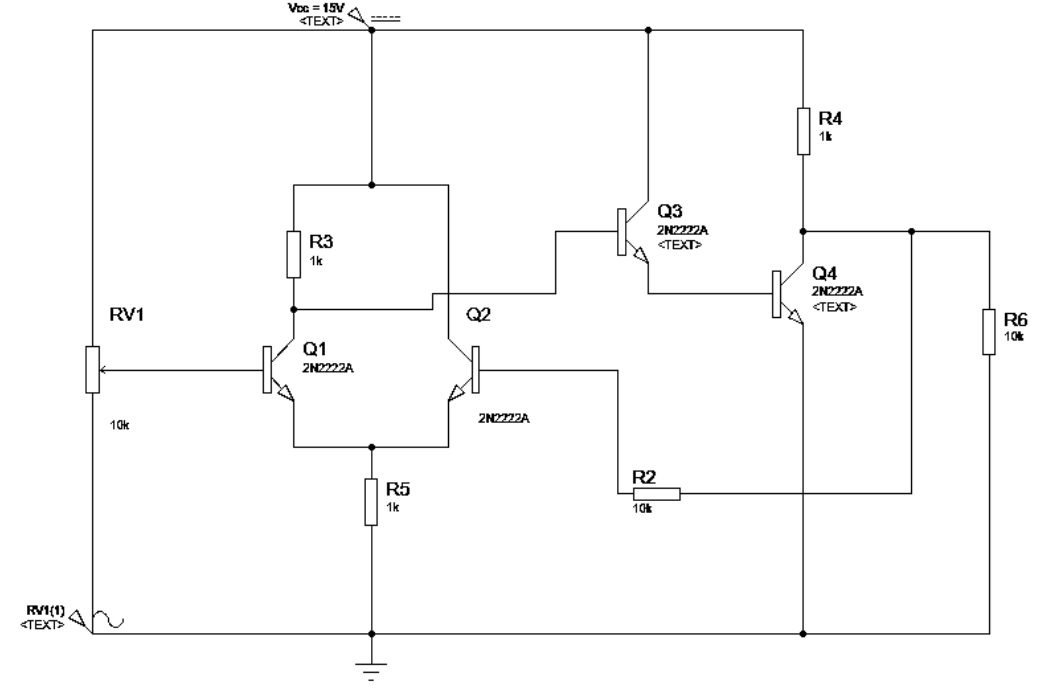
\includegraphics[width=0.5\textwidth]{media/circuito-dc.png}
        \caption{Amplificador diferencial con ganancia de corriente}
        \label{fig:circuito-inicial}
    \end{figure}
    
    Para poder determinar la respuesta del circuito frente a señales fue necesario analizar el circuito en su modelo en pequeña señal la cual se dividió en 2 partes (entrada y salida) teniendo en cuenta para ello el método de la fuente de prueba para representar este circuito mediante el desglose de la resistencia de retroalimentación en la entrada y salida del circuit, siendo el circuito de entrada del circuito el que se aprecia en la figura \ref{fig:psa}

    \begin{figure}[h]
        \centering
        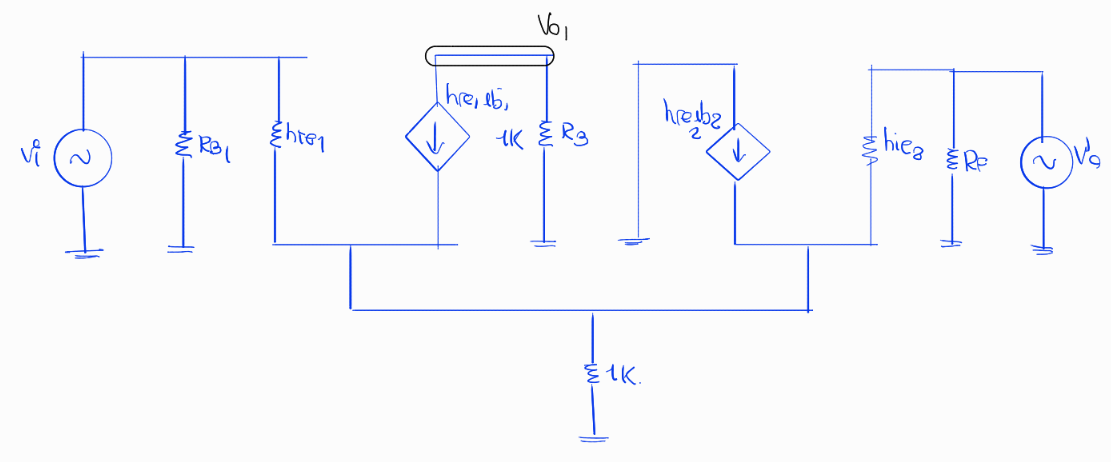
\includegraphics[width=0.5\textwidth]{media/modelo-pequena-senial-a}
        \caption{Modelo en pequeña señal de la entrada del circuito}
        \label{fig:psa}
    \end{figure}

    Por otro lado para el circuito de salida se tuvo en consideración el mismo reflejo de la resitencia de retroalimentación y la que se puede apreciar en la figura \ref{fig:psb}

    \begin{figure}[h]
        \centering
        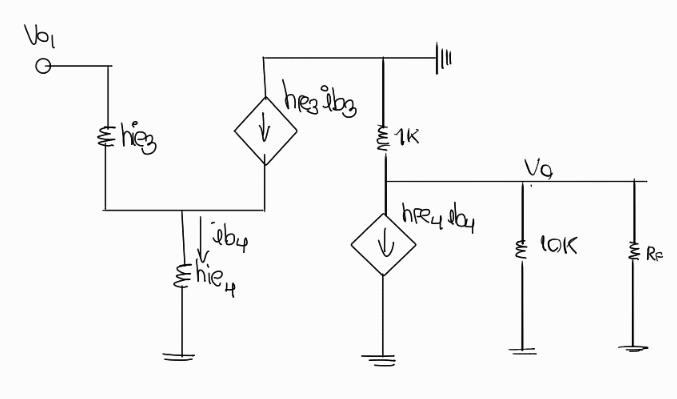
\includegraphics[width=0.4\textwidth]{media/psb}
        \caption{Modelo en pequeña señal de salida del circuito}
        \label{fig:psb}
    \end{figure}

    En función a los circuito mostrados se realizar el calculo de las respectivos parámetros de salida al relacionar la entrada y salida para la ganancia de voltaje y corriente y se hace uso de la fuente de prueba $V'_O$ para determinar el factor \textbf{T}.

    Para facilitar el análisis del circuito para diferentes valores se calculo una ganancia genérica en función a las características del circuito como la resistencia de entrada de cada transistor y las resistencias equivalentes producto del análisis en pequeña señal.

    \subsection{Calculo del factor de retroalimentación T}
    Para el cálculo de este valor se tuvo en cuenta la fuente de prueba $V'_O$ y la salida $V_O$ obteniendo tal relación mediante el empleo del voltaje $V_{O1}$ que se apreciar en la figura \ref{fig:psb}.

    Al realizar las equivalencias mediante las leyes electrícas se obtiene para el circuito de entrada de la figura \ref{fig:psa} que:

    \begin{equation}
        V_{01} = -hef_1*ib_1*R_3
		\label{eq:bucle-t-entrada}
	\end{equation}

    Y para el circuito de salida se tiene:

    \begin{equation}
        V'_O = -ib_1*(R_f+hie_1+hie_2 + RB_1)
		\label{eq:bucle-t-salida}
	\end{equation}

    Siendo así que para obtener T se realizo la relación entre las ecuaciones \ref{eq:bucle-t-entrada} y \ref{eq:bucle-t-salida} obteniendo finalmente:

    \begin{equation}
        \frac{V_O}{V_{01}} = \frac{-hie_4*R_{eq}*(1 + hfe_3)*hfe_1*R_3}{hie_3*(R_f+hie_1+hie_2 + RB_1)}
		\label{eq:t-resultado}
	\end{equation}

    Una vez definida la ganancia de retroalimentación se procedió a calcular la ganancia de voltaje del sistema $A_V$ con el objetivo de determinar la ganancia de retroalimentación regida por la siguiente ecuación definida en \cite{horenstein2000circuitos}

    \begin{equation}
        A_v = \frac{A_v}{1 - T}
		\label{eq:ganancia-av-fb}
	\end{equation}

    Y su equivalente para la ganancia de corriente de retroalimentación será:
    \begin{equation}
        A_i = \frac{A_i}{1 - T}
		\label{eq:ganancia-ai-fb}
	\end{equation}

    Al proseguir con el calculo se tiene que la ganancia de voltaje al relacionar la entrada y salida del circuito se tiene:

    \begin{equation}
        A_v = \frac{hie_3*R_eq*(1+hfe_3)*R_3*hfe_1}{hie_3^2*hie_1}
		\label{eq:ganancia-voltaje}
	\end{equation}

    De igual forma esta ganancia se calcula para la ganancia de corriente en retroalimentación y la cual por propia configuración del sistema se verá amplificada en gran medida debido a la configuración darlintong en la salida.

    
    \section{Paramétricos en pequeña señal para cada transistor: hie1, hie2, hie3 y hie4}

    La resistencia de entrada de cada transistor, se encuentra en función de la ganancia, el voltaje termico y la corriente $I_{CQ}$ determinada por la polarización CD del circuito.

    Siendo así que para este caso al considerar una resistencia de 8K en la entrada la ecuación general que se tendrá en cuenta para el calculo para cada resistencia de entrada del transistor 

    \begin{equation}
        hie_n = \frac{hfe_n*V_T}{I_{CQn}}
		\label{eq:resitencia-entrada-bjt}
	\end{equation}

    
    Las resistencias de entrada para cada transistor se apreciar en la tabla \ref{tb:hie-bjt} y de las cuales se puede observar que los transistores cuya resistencia de entrada es superior a los 100K $\Omega$ se encuentran en saturación debido a una mala polarización en los transistores.

    \begin{table}[]
        \begin{tabular}{|c|l|l|}
            \hline
            \textbf{Resistencia Entrada} & \multicolumn{1}{c|}{\textbf{$I_{CQ}$ {[}mA{]}}} & \textbf{hie {[}K$\Omega${]}} \\ \hline
            $hie_1$                        & 6.56                                       & 0.5945122            \\ \hline
            $hie_2$                        & 0.0274                                     & 142.335766           \\ \hline
            $hie_3$                        & 0.0354                                     & 110.169492           \\ \hline
            $hie_4$                        & 7.13                                       & 0.54698457           \\ \hline
        \end{tabular}
        \caption{Corriente de polarización y resistencia de entrada para cada transistor}
        \label{tb:hie-bjt}
    \end{table}
    
\section{Gráficas de polarización y puntos de operación}

    Se presenta la tabla \ref{fig:tabla-resumen-valores}, la cual contiene valores obtenidos a partir de la simulación del circuito en Multisim para los diferentes valores de resistencia definidos para la etapa de entrada en el transistor $Q_1$ que se apreciar en la figura \ref{fig:circuito-inicial}, siendo así que esta tabla nos brinda un visión general del comportamiento del circuito en función de los voltajes y corrientes obtenidas para determinar el función dentro de la región de activa o caso contrario.
    
    \begin{figure}[h]
        \centering
        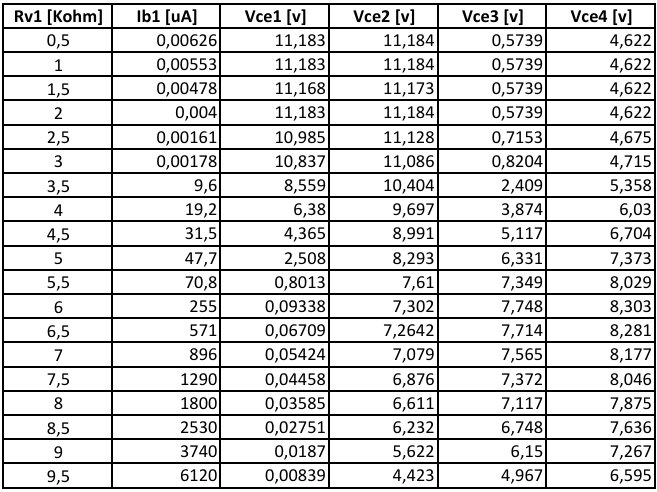
\includegraphics[width=0.5\textwidth]{media/IMAGENES MATLAB/TABLA1.png}
        \caption{Tabla de valores obtenidos en Multisim.}
        \label{fig:tabla-resumen-valores}
    \end{figure}

    Además en la tabla \ref{fig:tabla-resumen-valores} también se puede desglosar para analizar la variación el voltaje para cada resistencia configurada en la entrada siendo así que valores de resistencia entre los $4K\Omega$ y los $5.5K\Omega$ se pudo apreciar niveles de polarización adecuados para el correcto funcionamiento del circuito, sin embargo para que esto sea posible fue necesario agregar una resistencia de $200K\Omega$ en la base del transistor $Q_4$ la cual permitió limitar la corriente de control de $IB_4$ permitiendo el funcionamiento de tal transistor en su zona activa.
    
    \newpage

    En la figura \ref{fig:simulacion}, se puede apreciar tal modificación y mediante la cual se obtiene una salida no amplificada de la señal de entrada manteniendo su ganancia cerca de 1, en la figura también se puede apreciar el uso de un potenciómetro utilizado con la finalidad de poder calibrar la salida y poder ajustar dinamicamente el comportamiento del circuito durante su ejecución.

    \begin{figure}[h]
        \centering
        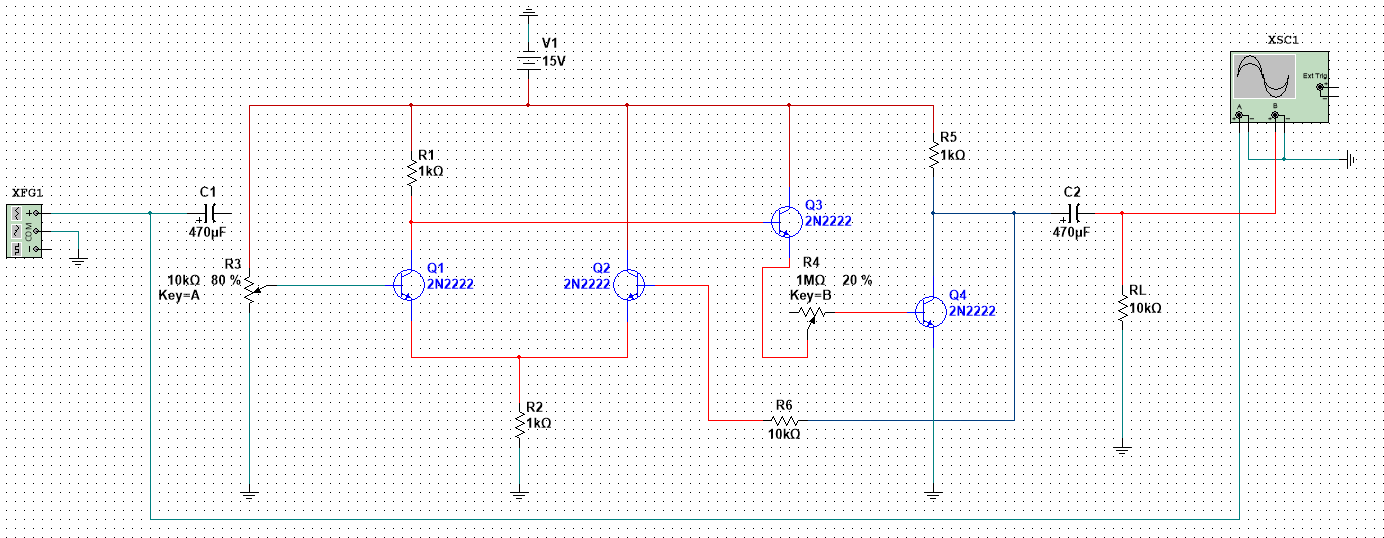
\includegraphics[width=0.5\textwidth]{media/simulacion.png}
        \caption{Simulación del amplificador retroalimentado - Multisim}
        \label{fig:simulacion}
    \end{figure}

    A continuación se muestran las gráficas y la evolución del voltaje y corriente en función de la resistencias de polarización de entrada $RV_1, RV_2$.
    
    \subsection{ Representación $I_{B1}$ vs $R_{v1}$}
    
    En la figura \ref{fig:Ib1} se observa que a medida que el valor de $R_{V1}$ se incremente, la corriente $Ib_1$ va creciendo de forma no lineal aproximándose la curva a una exponencial a causa del incremento de voltaje en el divisor de voltaje creado por el potenciómetro, siendo tal fenómeno el que causa la operación de los transistores fuera de la zona activa configurándolos en modo saturación.
    
    \begin{figure}[h]
        \centering
        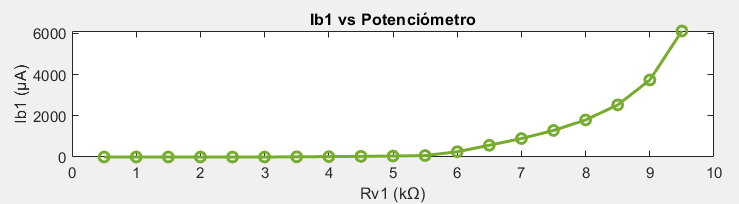
\includegraphics[width=0.5\textwidth]{media/IMAGENES MATLAB/IB1_R.png}
        \caption{$I_{B1}$ vs $R_{v1}$ }
        \label{fig:Ib1}
    \end{figure}
    
    \subsection{ Representación $V_{CE1}$ vs $R_{v1}$}
    Para valores bajos de RV1 , VCE1 se mantiene casi constante. A partir del punto 3.5Kohm VCE1 cae rápidamente.
    \begin{figure}[h]
        \centering
        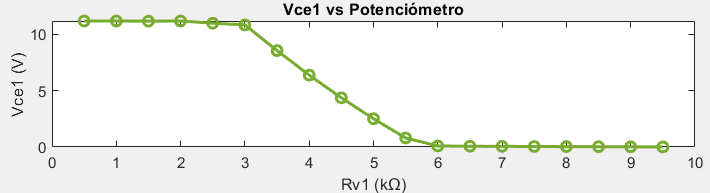
\includegraphics[width=0.5\textwidth]{media/IMAGENES MATLAB/VCE1_R.png}
        \caption{$V_{CE1}$ vs $R_{v1}$}
        \label{fig:Vce1}
    \end{figure}
    
    \subsection{ Representación $V_{CE2}$ vs $R_{v1}$}
    Semejante al caso anterior VCE2 semantiene casi constante y de la misma forma partir del punto 3.5kohm VCE2 cae. 
    \begin{figure}[h]
        \centering
        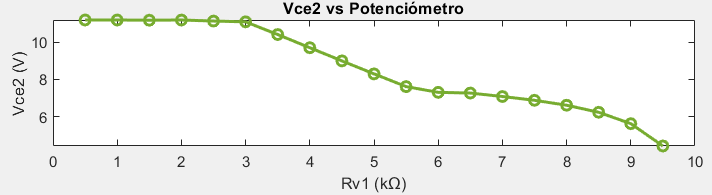
\includegraphics[width=0.5\textwidth]{media/IMAGENES MATLAB/VCE2_R.png}
        \caption{$V_{CE2}$ vs $R_{v1}$}
        \label{fig:vce2}
    \end{figure}
    
    \subsection{ Representación $V_{CE3}$ vs $R_{v1}$}
    VCE3 crece progresivamente.
    
    \begin{figure}[h]
        \centering
        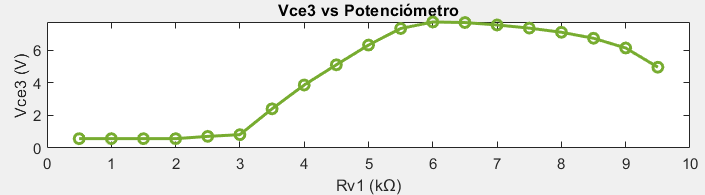
\includegraphics[width=0.5\textwidth]{media/IMAGENES MATLAB/VCE3_R.png}
          \caption{$V_{CE3}$ vs $R_{v1}$}
        \label{fig:vce3}
    \end{figure}
    
    \subsection{ Representación $V_{CE4}$ vs $R_{v1}$}
    De igual manera que el caso anterior VCE4 crece rápidamente.
    
    \begin{figure}[h]
        \centering
        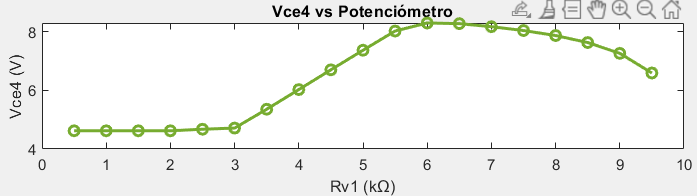
\includegraphics[width=0.5\textwidth]{media/IMAGENES MATLAB/VCE4_R.png}
          \caption{$V_{CE4}$ vs $R_{v1}$}
        \label{fig:vce4}
    \end{figure}
    
    \subsection{ Representación $V_{CR2}$ vs $R_{v1}$}
    VCR2 aumenta de manera notable  en cuanto Rv1 crece de colector.
    
    \begin{figure}[h]
        \centering
        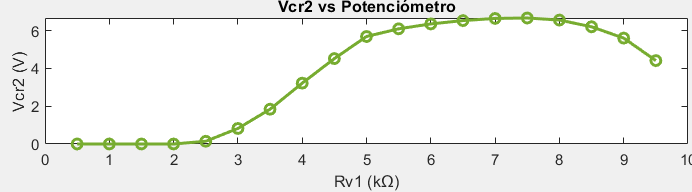
\includegraphics[width=0.5\textwidth]{media/IMAGENES MATLAB/VCR2_R.png}
        \caption{$V_{CR2}$ vs $R_{v1}$}
        \label{fig:vcr2}
    \end{figure}
    
    \newpage
    \subsection{ Representación $V_{CR4}$ vs $R_{v1}$}
    De igual forma se aprecia un cambio notable  al incrementar Rv1.
    \begin{figure}[h]
        \centering
        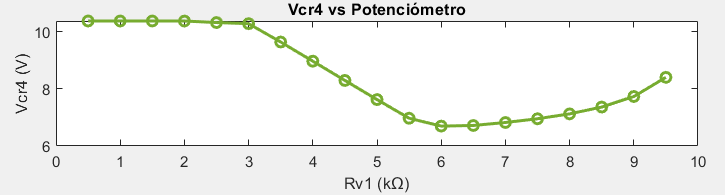
\includegraphics[width=0.5\textwidth]{media/IMAGENES MATLAB/VCR4_R.png}
        \caption{$V_{CR4}$ vs $R_{v1}$}
        \label{fig:vcr4}
    \end{figure}
    
    \subsection{ Representación $I_{CQ4}$ vs $R_{v1}$}
    
    \begin{figure}[h]
        \centering
        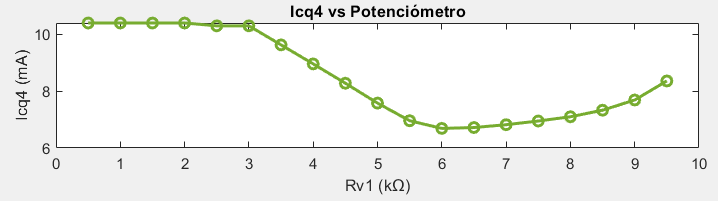
\includegraphics[width=0.5\textwidth]{media/IMAGENES MATLAB/ICQ4_R.png}
        \caption{$I_{CQ4}$ vs $R_{v1}$}
        \label{fig:Icq4}
    \end{figure}
    
    \section{Observaciones y conclusiones}
    \begin{itemize}
        \item El análisis en pequeña señal del amplificador diferencial permitió establecer un modelo preciso tanto en la entrada como en la salida, lo cual facilitó el cálculo del factor de retroalimentación $T$ mediante la aplicación del método de la fuente de prueba. Esto demuestra la importancia de descomponer el circuito en bloques funcionales para entender su comportamiento global.
    
        \item La ganancia del sistema, tanto en voltaje como en corriente, se encuentra fuertemente influenciada por el valor del factor de retroalimentación $T$, siendo evidente que configuraciones como la Darlington en la etapa de salida amplifican significativamente la respuesta de corriente, lo cual es útil en aplicaciones donde se requiere gran capacidad de entrega de corriente a la carga.
    
        \item El cálculo de los parámetros en pequeña señal para cada transistor mostró que una incorrecta polarización puede llevar a niveles de resistencia de entrada anormalmente altos, lo cual indica que algunos transistores podrían estar en saturación. Este resultado resalta la importancia de una adecuada polarización DC para garantizar un funcionamiento lineal y eficiente del amplificador.
    \end{itemize}

    
	
	% Contenido del documento
	
	
	\bibliographystyle{IEEEtran}
	\bibliography{biblio}
\end{document}